
\begin{slide}{Why we use X-rays to study atoms}

 \begin{cenpage}{150mm}

  X-rays are light with wavelength $\lambda:  [ 0.05 : 50] {\rm\,\AA} $
  or  energy $E : [ 0.25 - 250]  \rm\,keV$.

  \vmm\vmm
  
  
{\only<1>{ 
     
     \begin{columns}
       \begin{column}{60mm}
         X-rays are used in many scientific fields for studying:
         \vmm
         
           \begin{itemize}
           \item interior micro-structure of materials.
           \item atomic-scale structure of materials.
           \item chemical composition of materials.
           \item chemical state of elements.
           \end{itemize}
         \end{column}
         \begin{column}{1mm}
         \end{column}
         \begin{column}{90mm}            
            \includegraphics[width=90mm]{figs/images/em_spectrum}
         \end{column}
       \end{columns}
       
}}
  

{\only<2,3>{

      X-rays have 3 main properties:

  \vmm
  {\small\bf{
  \begin{tabular}{lll}
    {\Red{Property}}   &
    Behavior   &
    {\Blue{Use}} \\
    \noalign{\medskip}    \hline   \noalign{\medskip}
    \begin{minipage}{40mm}
 {\Red{Interact weakly with electrons}}
    \end{minipage}&
    \begin{minipage}{52mm}
      penetrate deeply into matter, with
      {\emph{strong contrast in  atomic number $Z$}}.
    \end{minipage}&
      {\Blue{Imaging, Tomography}}    \\
    \noalign{\bigskip}
    \begin{minipage}{21mm}
    {\Red{Energy}}
    \end{minipage}&
    \begin{minipage}{48mm}
     comparable to binding energies of core electrons in atoms.
    \end{minipage}&
      {\Blue{Spectroscopy}}    \\
    \noalign{\bigskip}
    \begin{minipage}{21mm}
    {\Red{Wavelength}}
    \end{minipage}&
    \begin{minipage}{48mm}
      comparable to distances between atoms in solids and liquids.
    \end{minipage}&
      {\Blue{Scattering, Diffraction}}    \\
    \noalign{\medskip}
    \hline
  \end{tabular}

}}}}

\vmm\vmm

{\onslide+<3->{

    X-rays from synchrotron sources also have these properties,
    that can be useful for many %% imaging, scattering, and spectroscopy
    applications:

     \begin{itemize}
       \item highly  {\RedEmph{polarized}} in the horizontal plane.

       \item highly  {\RedEmph{collimated}} and so possible to focus to
         beams at $\rm {\mu}m$ or nanometer scale.

       \item partially {\RedEmph{coherent}} - being ``in phase'' with
         other X-rays.
       \end{itemize}

\begin{postitbox}{65mm}
  We will focus on the Energy property of X-rays.
\end{postitbox}
}
}

\vspace{10mm} \vfill
\end{cenpage}
\end{slide}

%%%%%%%%%%%%%%%%%%%%%%5


\begin{slide}{X-ray Penetration and Imaging}

  \begin{cenpage}{150mm}

    X-rays penetrate deeply into matter, with strong dependence on  X-ray
    energy and  material composition.
  
 \vmm\vmm
  
     
     \begin{columns}
       \begin{column}{55mm}

         X-rays are {\RedEmph{attenuated}} by matter as
         
         \begin{postitbox}{18mm}
           {  $ \displaystyle  I = I_0 e^{-\mu t} $   }
         \end{postitbox}


       Where
       \begin{itemize}
       \item[$I$]       X-ray intensity after material
       \item[$I_0$]    X-ray intensity before material
       \item[$t$]        material thickness
       \item[$\mu$]    absorption coefficient
       \end{itemize}

       \vmm\vmm

       \hspace{7mm} \includegraphics[width=40mm]{figs/rimg/beer_lambert}
       
         \end{column}
         \begin{column}{1mm}
         \end{column}
         \begin{column}{75mm}
           \onslide+<2-> {

           \begin{columns}
             \begin{column}{35mm}
               \includegraphics[height=43mm]{figs/images/XrayHand}
               
               {\small {
                   \vmm
                   Early X-ray image of hand with wedding ring (1896).
                 }}
               
             \end{column}
             \begin{column}{35mm}            
               \includegraphics[height=43mm]{figs/images/Roentgen}
               
               {\small {
                   \vmm
                   Wilhelm Conrad Roentgen: discovered X-rays (1895).
                 }}
               
             \end{column}          
           \end{columns}
      
         \vmm \hrule \vmm \vmm

         X-rays  penetrate flesh.
         
         X-rays are partially stopped by bone.
         
         X-rays are almost completely stopped by metal ring.
         }
         
       \end{column}          
     \end{columns}


\vspace{10mm} \vfill

\end{cenpage}
\end{slide}

\begin{slide}{The X-ray Attenuation Coefficient: $\mu$ in $I = I_0 e^{-\mu t}  $}

  \begin{cenpage}{125mm}
    Three processes cause attenuation: 1) Rayleigh (elastic) scattering, 2)
    Compton (inelastic) scattering, and 3) the photo-electric effect or
    {\RedEmph{X-ray absorption}}.
    
  \vmm

  For heavy elements and moderate X-ray
  energies, photo-electric absorption dominates.
  \vmm
  
  \end{cenpage}
      

  \begin{columns}[T]
    \begin{column}{45mm}

      \vmm

      The photo-electric portion of $\mu$, depends linearly on
      density, {\Blue{$\rho$}}, and very strongly on
      
      \begin{itemize}
      \item   atomic number,  {\Blue{$Z$}}.
      \item   X-ray energy,  {\Blue{$E$}}.
      \end{itemize}
          
      \vmm

      \begin{postitbox}{30mm}      
      {\Large{
      \[ {\Blue{ \mu \sim \frac{\rho Z^4}{ E^3} }} \]
    }}
  \end{postitbox}
  
    \end{column}
    \begin{column}{105mm}
      
      \includegraphics[width=90mm]{figs/general/murho_total}


    \end{column}
  \end{columns}

\begin{cenpage}{130mm}
  $\mu$ has sharp {\RedEmph{Absorption Edges}} at the characteristic
  core-electron energy levels of each atom.
\end{cenpage}

\vmm
\vfill

\end{slide}



\begin{slide}{The X-ray Attenuation Coefficient: Compton and Rayleigh Scattering}

  \begin{cenpage}{125mm}
    Three processes cause attenuation: 1) Rayleigh (elastic) scattering, 2)
    Compton (inelastic) scattering, and 3) the photo-electric effect or
    {\RedEmph{X-ray absorption}}.
    
  \vmm

  For heavy elements and moderate X-ray
  energies, photo-electric absorption dominates.
  \vmm


  \vmm
  For light elements at high energy Compton scattering can dominate.
  \vmm


  
  \end{cenpage}
      

  \begin{columns}[T]
    \begin{column}{65mm}

      \includegraphics[width=55mm]{figs/general/mu_xsections_O}
  
    \end{column}
    \begin{column}{65mm}
      
      \includegraphics[width=55mm]{figs/general/mu_xsections_Fe}

    \end{column}
  \end{columns}

\begin{cenpage}{130mm}
  $\mu$ has sharp {\RedEmph{Absorption Edges}} at the characteristic
  core-electron energy levels of each atom.
\end{cenpage}

\vmm
\vfill

\end{slide}

\begin{slide}{X-Ray Absorption and the Photo-Electric Effect}

  \begin{cenpage}{90mm}
    X-rays are absorbed by all matter through the {\RedEmph{photo-electric
        effect}}:
  \end{cenpage}

  \begin{columns}[T]
    \begin{column}{50mm}

      
      \vspace{8mm}

      An atom absorbs an x-ray when the x-ray energy is transferred to a
      core-level electron ({\sl{K}}, {\sl{L}}, or {\sl{M}} shell).
      
      \vmm\vmm
      
      The atom is left in an {\RedEmph{excited state}} with a {\RedEmph{core
          hole}} -- an empty electronic level.
      
      \vmm
      Any excess energy from the x-ray is given to an
      ejected {\RedEmph{photo-electron}}.

      \vmm
            \vmm

            
        \begin{columns}
          \begin{column}{8mm}
            \rgraph{8mm}{Einstein}
          \end{column}
          \begin{column}{40mm}

            {\tiny{A. Einstein, Nobel Prize, 1921 ``For his services to Theoretical Physics, and
               especially for his discovery of the law of the photoelectric
               effect''.}}

           \vfill
           
          \end{column}
        \end{columns}

      \end{column}
      \begin{column}{66mm}
        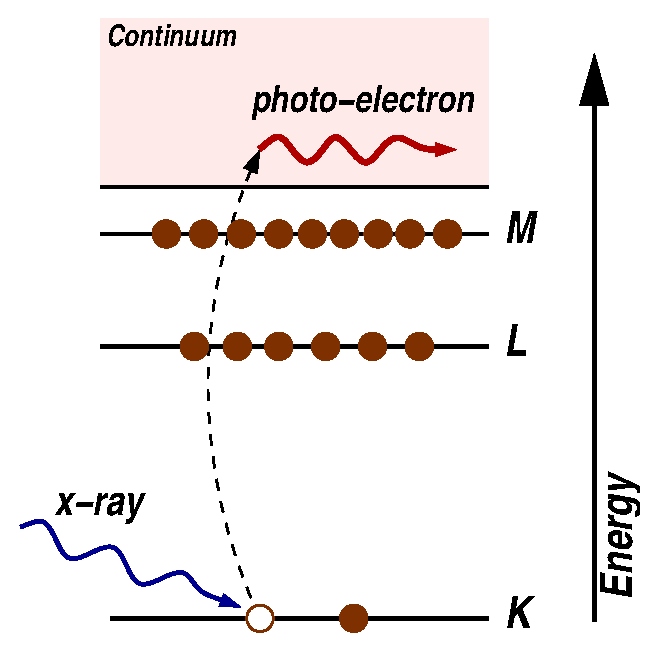
\includegraphics[width=65mm]{figs/rimg/photoelectric}

        \vmm  \vfill
      \end{column}
    \end{columns}

    \vmm
    \vfill
\end{slide}


\begin{slide} {X-ray Fluorescence and Auger emission}

\begin{cenpage}{110mm}
  After X-ray absorption, the excited atom relaxes to the
  ground state.  A higher level electron fills the core hole, and a
  {\RedEmph{fluorescent X-ray}} or {\RedEmph{Auger electron}} is emitted.
\end{cenpage}

\vmm

  \begin{columns}[T]
      \begin{column}{55mm}
        {\RedEmph{X-ray Fluorescence}}:
        Emit an X-ray with energy given by core-levels energies.

       \hspace{4mm} \rgraph{38mm}{xray_emission_fluor}

        \begin{columns}
          \begin{column}{8mm}
            \rgraph{8mm}{Barkla}
          \end{column}
          \begin{column}{40mm}

            {\tiny{Charles Barkla, Nobel Prize, 1917 ``discovery of the characteristic R\"ontgen radiation of the elements"
                }}
          \end{column}
        \end{columns}

      \end{column}
      \begin{column}{55mm}
        \onslide+<2->

        {\RedEmph{Auger Effect}}:
        Promote an electron from another core-level to the continuum.

       \hspace{4mm} \rgraph{38mm}{xray_emission_auger}

        \begin{columns}
          \begin{column}{8mm}
            \rgraph{8mm}{Meitner}
          \end{column}
          \begin{column}{40mm}

            {\tiny{Lise Meitner, no Nobel Prize,  first to discover Auger effect, explained nuclear fission}}.

          \end{column}
        \end{columns}

      \end{column}
    \end{columns}

    \onslide+<3->

    \begin{postitbox}{105mm}
        X-ray fluorescence and Auger emission have discrete energies,
        characteristic of the absorbing atom -- very useful for identifying atoms!
      \end{postitbox}

\vfill
\end{slide}

\begin{slide} {X-ray Fluorescence (XRF) Spectroscopy}

  \begin{cenpage}{140mm}

    {\ }

    \begin{columns}[T]
    
      \begin{column}{68mm}
        
        The fluorescence X-rays at characteristic energies from different
        elements can be used to identify element and to quantify elemental
        abundances often down to ppm levels.

      \vmm\vmm
      
      \includegraphics[width=62mm]{figs/images/XRF_Spectrum}

      \vmm \vfill

      \vspace{27mm}
      \vfill
      
    \end{column}

      \begin{column}{2mm}    
      \end{column}
    
    \begin{column}{69mm}            

      In a modern electron-probes and X-ray microprobe beamlines, XRF
      spectra are collected fast enough to make elemental maps in a few hours.

      \vmm
      
      \hspace{3mm} \includegraphics[width=55mm]{figs/images/XRF_Map1}

      {\DarkRed{K}} / {\DarkGreen{Mn}} / {\BrightBlue{Zn}} from a
      hyper-accumulating plant grown in two different conditions.

      \vmm

      Map size: 10 x 9 mm,  pixel size: 5 $\rm{\mu}m$.

      15 ms per pixel.

      \vspace{10mm}
      \vfill
    \end{column}
    \end{columns}
    


\end{cenpage}

\end{slide}





\begin{slide}{X-ray Absorption Spectroscopy:  EXAFS and XANES.}

  \begin{cenpage}{102mm}

    X-ray Absorption Spectroscopy ({\Blue{XAS}}) is the modulation of
    the X-ray absorption coefficient at energies at and above an X-ray
    absorption edge.

    \vmm
    \begin{center}
      \begin{tabular}{ll}
        {\Blue{XAFS}} &  X-ray Absorption Fine-Structure Spectroscopy  (= XAS) \\
        {\Blue{XANES}} & X-ray Absorption Near-Edge Spectroscopy\\
        {\Blue{EXAFS}} & Extended X-ray Absorption Fine-Structure \\
      \end{tabular}
    \end{center}
    \vspace{1mm}

    These contain information about an element's chemical state (XANES) and
    local atomic environment (EXAFS).

    \end{cenpage}

    \vspace{2mm}

    \begin{columns}[T]
      \begin{column}{58mm}
         \rgraph{60mm}{mu_xanes_exafs}
         \vspace{-2.5mm} {\hspace{8mm} \tiny{Fe {\slshape{K}}-edge XAFS for FeO.}}
      \end{column}
      \begin{column}{65mm}
        {\RedEmph{Main XAS Characteristics}}:
        \begin{itemize}
        \item local atomic coordination
        \item valence, oxidation state
        \item applies to any element ($Z > 2$) .
        \item works at low concentrations (ppm, $\mu$M)
        \item minimal sample requirements.
        \item independent of crystal  structure, isotope.
        \end{itemize}
      \end{column}
    \end{columns}

\vfill
\end{slide}

\begin{slide}{XANES:  X-ray Absorption Near-Edge Spectroscopy}
\begin{cenpage}{120mm}
 Within $\sim$100eV of the absorption edge, the X-ray Absorption Spectra is
 highly sensitive to the chemical state and formal valence of absorbing element:
\end{cenpage}

\begin{cenpage}{150mm}
  \vmm
  \begin{columns}
    \begin{column}{48mm}
      \includegraphics[width=48mm]{figs/xanes/cr}

      \vmm
      \hspace{5mm}  $\rm Cr^{3+}$ and $\rm Cr^{6+}$
    \end{column}
    \begin{column}{48mm}    
      \includegraphics[width=48mm]{figs/xanes/as}
      
      \vmm
      \hspace{5mm}    $\rm As^{3+}$ and $\rm As^{5+}$
    \end{column}

    \begin{column}{48mm}
     \includegraphics[width=48mm]{figs/xanes/fe_oxides}
      \hspace{5mm}    Fe metal and oxides.
    \end{column}
  \end{columns}

  \vmm
  
    The oxidation state and local atomic coordination environment strongly
    affect the lowest unfilled electronic levels of an absorbing atom.

    \vmm
    \begin{center}
      
    \begin{postitbox}{105mm}
        {\BlueEmph{what are the unoccupied electronic states
            that the photo-electron can fill?}}
    \end{postitbox}
  \end{center}

  \end{cenpage}

\vfill
\end{slide}


 \begin{slide}{EXAFS: Extended X-ray Absorption Fine Structure}

 \begin{cenpage}{112mm}
   Even far above the edge, there are oscillations in $\mu(E)$ that are
   sensitive to the positions and types of atoms neighboring the absorbing
   atom.
 \vmm

  We define the EXAFS as:

   \[
   \mu(E) =   \mu_0(E) [1 + \chi(E)]  \hspace{15mm} \chi(E) =   \frac{ {\mu(E) - \mu_0(E)}}{\Delta \mu_0(E_0)}
   \]

   We subtract off a smooth {\BlueEmph{``bare atom'' background}}
   $\mu_0(E)$, and divide by the {\BlueEmph{``edge step''}}
   $\Delta \mu_0(E_0)$ to get $\chi$, the EXAFS oscillations:


 \begin{tabular}{ll}
   \onslide+<1->
   \begin{minipage}{55mm}
     \rgraph{55mm}{mu_with_mu0}
   \end{minipage}
   &
   \onslide+<1->
   \begin{minipage}{55mm}
     \rgraph{55mm}{chie}
   \end{minipage} \\
    \noalign{\smallskip}\\
   \onslide+<1->
   \hspace{3mm} $\mu(E)$ and $\mu_0(E)$ for FeO
   &
   \onslide+<1->
   \hspace{3mm} $\chi(E)$ for FeO, with $E_0$ = 7122 eV.
 \end{tabular}

  \end{cenpage}

 \vfill
\end{slide}


\begin{slide}{Using X-ray wavelength: X-ray Scattering and Diffraction}

   \begin{columns}[T]
   \begin{column}{75mm}

     The spacing between atoms in most molecules, solids, and liquids is
     typically 1 to 10 {\AA}.

    \vmm
     X-rays have the right wavelengths to scatter
     (Rayleigh or elastic scattering) from planes of atoms coherently.
     \vmm
     
     \includegraphics[width=67mm]{figs/images/XRD_Scatter}

     \vmm
     \includegraphics[width=67mm]{figs/images/XRD_diffract}

     \end{column}

     \begin{column}{47mm}

       \includegraphics[width=38mm]{figs/images/XRD_XTAL}

       
       When the X-ray are at the right angle, the scattered X-rays with
       constructively interfere to diffract.

       \vmm
 
       This can be used to tell the spacing between atoms.
       
     \end{column}
    \end{columns}

    \begin{postitbox}{80mm}
      Diffraction is the most common use of synchrotron X-rays
    \end{postitbox}

 \vfill
\end{slide}     

\begin{slide}{Using X-ray wavelength: X-ray Diffraction}

   \begin{columns}[T]
     \begin{column}{80mm}


       X-rays with the right wavelengths and angle of incidence to a
       crystal can diffract according to Bragg's law:

       \begin{center}
         \begin{postitbox}{28mm}
           {\Large{
               $  n\lambda = 2 d \sin(\theta) $
             }}
         \end{postitbox}
         \end{center}


       Where
       \begin{itemize}
       \item[$\lambda$]       X-ray wavelength
       \item[$d$]    spacing between atomic planes
       \item[$\theta$]        scattering angle
       \end{itemize}
         
     
     \includegraphics[width=64mm]{figs/images/XRD_Pattern}

     X-ray diffraction pattern for Fe3C
     
     \end{column}

     \begin{column}{47mm}

       \begin{columns}[T]
         
         \begin{column}{20mm}         
           \includegraphics[width=18mm]{figs/images/WLBragg}

           William L. Bragg (son)
           
           \vmm
           \vmm
           
           All Nobel prize winners for work on X-ray diffraction.
           
         \end{column}
         
         \begin{column}{20mm}         
           \includegraphics[width=18mm]{figs/images/WHBragg}
           
           William H. Bragg (father)
           
           \vmm
           \vmm
           
           \includegraphics[width=18mm]{figs/images/MaxvonLaue}
           
           Max von Laue        
          
          \end{column}
       \end{columns}


     \end{column}
   \end{columns}

 \vfill
\end{slide}     


\begin{slide}{X-ray Diffraction at synchrotrons}

  \begin{cenpage}{110mm}
    These days, X-ray diffraction at synchrotrons is done on

     \begin{itemize}
     \item very large molecules (proteins).
     \item on samples at extreme conditions (high pressure, high
       temperature).
     \item on very disordered materials (liquids, surfaces, interfaces).
     \item at very high speed to see dynamics.
     \item at very small scales and high-precisions to measure strain.
       \end{itemize}

     \end{cenpage}
     
       \begin{columns}[T]
         \begin{column}{65mm}
           \includegraphics[width=45mm]{figs/images/XRD_MacroPattern}

           X-ray Diffraction Pattern from Macro-molecule.
           
         \end{column}
         \begin{column}{75mm}
           \includegraphics[width=45mm]{figs/images/XRD_MacroMolecule}

           Molecular structure solved with X-ray Diffraction.

         \end{column}         

     \end{columns}
 \vfill
\end{slide}     
